\documentclass[a4paper]{llncs}
\usepackage[latin1]{inputenc}
\usepackage{amsmath}
\usepackage{amssymb}
\usepackage[algo2e]{algorithm2e}
\usepackage{pgf}
\usepackage{tikz}
\usepackage{verbatim}
\usetikzlibrary{arrows,automata}
\usepackage{graphicx}
\usepackage{sidecap}
%% \usepackage{caption}
\usepackage{subcaption}

\usepackage{url}
\urldef{\mailsa}\path|cs1090197@cse.iitd.ac.in|

\setcounter{tocdepth}{3}
%% \setcounter{lofdepth}{1}

\begin{document}

\mainmatter

\title{Tools and Algorithms for Deciding Relations on Timed Automata}

\author{Mihir Mehta}

\institute{Department of Computer Science and Engineering,\\
  Indian Institute of Technology, Delhi.\\
  \mailsa\\
}

%% \date{April 2013}

\maketitle

\begin{abstract}
  This describes the author's work in implementing the construction of
  zone-valuation graphs for timed automata and using these to verify
  certain relations on pairs of timed automata.
  Timed automata are a widely-used formalism, in verification, for
  describing systems where the execution is subject to timing
  constraints. One area of interest is the verification of certain
  timed and time abstracted relations on pairs of timed automata,
  which are generally of either an equivalence nature or a
  pre-ordering nature. Among existing tools, minim
  \cite{tripakis2001analysis} serves to verify certain of these
  relations, but it is limited in its scope and fails to meet certain
  requirements of reachability in its output. We build upon the work
  of \cite{DBLP:conf/cav/GuhaNA12}, in which algorithms for building
  zone-valuation graphs (minimal, discrete equivalent representations
  of timed automata) are given and used to verify certain pre-ordering
  relations on pairs of timed automata. We present an modified version
  of the zone-valuation graph construction algorithm, and a
  generalisation of the algorithm which uses zone-valuation graphs to
  verify a larger set of timed and time-abstracted relations on timed
  automata, where this generalisation builds upon the work of
  \cite{arun2006bisimilarities}. We also describe a reference
  implementation of these algorithms in Ocaml.
\end{abstract}
% timed automata - formalism for automata with timing
% constraints. time abstracted relations. decidable using region
% graphs. our tool checks for the existence of various kinds of timed
% relations between timed automata using a zone-based. approach. 
\pagebreak

\tableofcontents
\pagebreak
\listoffigures
\pagebreak

\section{Introduction}

The work described in this thesis builds on the work of
\cite{DBLP:conf/cav/GuhaNA12} in which Guha et al described an
algorithm to generate \emph{zone valuation graphs} for timed automata
and an algorithm to use such zone-valuation graphs to determine
\emph{timed performance prebisimilarity} on pairs of timed
automata. Our aim was to implement these algorithms in a generalised
manner in order to verify various other time abstracted relations,
such as time abstracted bisimulations \cite{tripakis2001analysis} and
time abstracted simulation equivalence. Towards
this end, we studied the literature about timed automata as well as
various existing tools for verifying these
equivalences (such as \texttt{minim}, described in
\cite{tripakis2001analysis}). Our implementation, in OCaml, implements
several of these relations and leaves some scope for implementing
others.

This document proceeds by developing the relevant theory for labelled transition
systems and strong bisimilarity, and then continues with timed
automata and time abstracted bisimilarity in analogous fashion. We 
then detail several methods to discretise the state space of timed
automata, including region graphs, zone graphs, and zone valuation
graphs, and use region graphs to show that a finite representation of
the state space of a timed automaton is always decidable. We mention
difference bound matrices (DBM), a widely used representation for the time
constraints (i. e. convex polyhedra) that are used to describe
zones. Then, we explain abstractions, which are transformations on DBM
that replace each DBM by a DBM which is its superset and
which is equivalent to it modulo strong time abstracted
bisimilarity. This helps us prevent state space explosion in our
exploration algorithms which build the state space of a timed
automaton. We then explain the common features of certain time
abstracted relations which allow us to verify them in a generalised
manner, and explain our implementation.

%Include the organisation of the thesis.

\section{Labelled transition systems}

\begin{SCfigure}
  \centering
  \def\svgwidth{0.3\columnwidth}
  \input{lts01.pdf_tex}
  \caption{An example of a labelled transition system. Here, the
    states are $\{0, 1, 2, \ldots 7\}$ and the actions are $\{0,
    1\}$.}
  \label{lts01}
\end{SCfigure}

\begin{definition}
  \emph{Labelled Transition System}: A labelled transition system (LTS)
  \cite{Keller:1976:FVP:360248.360251} is an automaton which is
  described by
  \begin{itemize}
  \item $S$, a set of \emph{states} 
  \item $Act$, a set of \emph{actions}
  \item $\rightarrow \subseteq S \times Act \times S$, a \emph{transition
    relation}.
  \item optionally, $I \subseteq S$ ,a set of initial states. If there
    is exactly one initial state, then the LTS is said to be \emph{rooted}.
  \end{itemize}
\end{definition}

LTS are useful for describing the behaviour of untimed systems, and
serve as the foundation for the development of more complex models
such as CCS and timed automata. Thus, equivalences on LTS serve
as the theoretical foundation for many timed and time abstracted
equivalences on timed automata, and also have direct applications in
determining some of these equivalences in cases where timed automata
can be reduced to equivalent LTS.

\section{Equivalences on labelled transition systems}

\subsection{Strong bisimilarity}

\begin{SCfigure}
  \centering
  \def\svgwidth{0.5\columnwidth}
  \input{lts01quotient.pdf_tex}
  \caption{Strong bisimilarity quotient of the LTS in Figure~\ref{lts01}.}
\end{SCfigure}

A binary relation $R$ is a \textit{strong
  bisimulation} if and only if, for all $(s_1, s_2)$ $\epsilon$ $R$ and $a$ $\epsilon$ $Act .$\\
$\forall s_1' (s_1 \xrightarrow{a} s_1' \Rightarrow \exists s_2'
. (s_2 \xrightarrow{a} s_2' \wedge (s_1', s_2')$ $\epsilon$ $R ) )
\wedge $ \\
$\forall s_2' (s_2 \xrightarrow{a} s_2' \Rightarrow \exists s_1'
. (s_1 \xrightarrow{a} s_1' \wedge (s_1', s_2')$ $\epsilon$ $R ) )$

It can be shown that the union of
all strong bisimulations over the set of states is a strong
bisimulation. This binary relation is called \textit{strong
  bisimilarity}, denoted by $\sim$.

Strong bisimilarity between two states in an LTS implies,
intuitively, that any action performed by the one can be performed by
the other and vice versa.

An algorithm to evaluate strong bisimilarity was first given by
Kanellakis and Smolka \cite{kanellakis1990ccs}. A faster algorithm for
the special case having just one kind of action was given by Paige and
Tarjan \cite{paige1987three} and made general by Fernandez
\cite{fernandez1990implementation}.

\section{Clocks, valuations and related operations}

The timing model we use relies on the notions of clocks and
valuations. The timing information about the possible executions of a
timed automaton can, intuitively, be expressed in terms of constraints
on clocks. We will make this idea more precise as we go on.

\begin{definition}
\emph{Clock}: A clock is a variable ranging over the set of
non-negative real numbers, $R_{\geq 0}$.
\end{definition}

\begin{definition}
\emph{Valuation}: A valuation over a set of clocks $C$ is a
function $C \rightarrow R_{\geq 0}$, assigning non-negative values
to each of the clocks.
\end{definition}

Two important operations on clock valuations are clock resets and
delays. For a subset $X$ of $C$, the clock reset of a valuation $v$
is given by
\begin{displaymath}
  v[X:=0](x) = 
  \begin{cases}
    0    & \text{if } x \epsilon X \\
    v(x) & \text{if } x \epsilon C - X
  \end{cases}
\end{displaymath}

For a real delay $d$ $\epsilon$ $R_{\geq 0}$, the delay of a valuation
$v$ is given by
\begin{displaymath}
  (v + d)(x) = v(x) + d \quad \forall x \epsilon C
\end{displaymath}

\begin{definition}
\emph{Hyperplane}: Expressions of the forms $x \smile c$ and $x - y
\smile c$, where $x, y \epsilon C$, c is an integer, and $\smile
\epsilon \{ <, \leq, \geq, >\}$ are known as \emph{atomic clock
  constraints}. A valuation $v$ over $C$ is said to satisfy the
atomic clock constraint $x \smile c$ if $v(x) \smile c$ and $x - y
\smile c$ if $v(x) - v(y) \smile c$. A hyperplane is a set of
valuations satisfying an atomic clock constraint.
\end{definition}

\begin{definition}
\emph{Polyhedron}: The set of polyhedra over a set of clocks $C$ is
the smallest subset of the set of all valuations over $C$ that 
\begin{itemize}
\item contains all hyperplanes over C
\item is closed over intersection, union and complementation.
\end{itemize}
\end{definition}

\begin{definition}
\emph{Convex polyhedron}: A convex polyhedron is a polyhedron that can
be represented as the intersection of a set of hyperplanes.
\end{definition}

It should be noted that this definition does not coincide exactly with
the notion of a convex set from algebra. For instance, for
$C=\{x_1, x_2\}$, the set $\{(x_1, x_2)| x_1 \geq 0, x_2 \geq 0, x_1 +
x_2 > 0\}$ is convex but not a convex polyhedron.

Union, intersection, complementation and set difference are well
defined operations on polyhedra, but of these, intersection is the
only operation which preserves convexity.

The \emph{pre-reset} and \emph{post-reset} of a set $X$ $\epsilon$ $C$ on a
polyhedron $\zeta$ over the set $C$ of clocks are respectively defined
by
\begin{align*}
[X := 0]\zeta &= \{v| v[X := 0] \epsilon \zeta \} \\
\zeta[X := 0] &= \{v[X := 0]| v \epsilon \zeta \}
\end{align*}

The \emph{future} of a polyhedron $\zeta$ over a set $C$ of clocks
is given by 
\begin{displaymath}
\zeta \uparrow = \{v + d| v \epsilon \zeta, d \epsilon R_{\geq 0}\}
\end{displaymath}

The operators intersection, future, pre-reset, post-reset and future
preserve convexity of polyhedra.

\begin{definition}
\emph{Clock constraint}: A clock constraint is a polyhedron which can
be expressed as an intersection of hyperplanes of the form $x \smile
c$.
\end{definition}

A related term, \emph{extended clock constraint}, can be used
interchangeably with \emph{polyhedron}.

\section{Timed automata}

\begin{SCfigure}
  \centering
  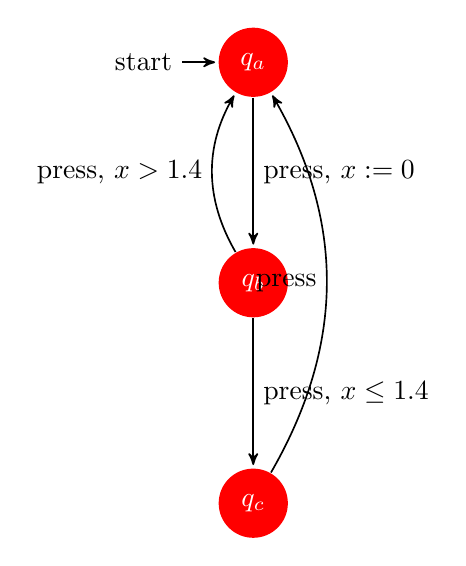
\begin{tikzpicture}[->,>=stealth',shorten >=1pt,auto,node
      distance=2.8cm,
      semithick]
    \tikzstyle{every state}=[fill=red,draw=none,text=white]

    \node[initial,state] (A)                    {$q_a$};
    \node[state]         (B) [below of=A] {$q_b$};
    \node[state]         (C) [below of=B] {$q_c$};
    
    \path (A) edge              node {press, $x:=0$}    (B)
    (B) edge [bend left] node {press, $x > 1.4$}        (A)
    edge              node {press, $x \le 1.4$}         (C)
    (C) edge [bend right] node {press}                  (A);
  \end{tikzpicture}

  \caption{Timed automaton representing a light bulb with two
    brightness settings, example taken from \cite{aceto2007reactive}}
\end{SCfigure}

\begin{definition}
  \emph{Timed Automaton}: A timed automaton
  \cite{Alur94atheory} over a finite set of clocks $C$
  and a finite set of actions $Act$ is a 4-tuple $(L, l_{0}, E, I)$.
  \begin{itemize}
  \item $L$ is a finite set of locations.
  \item $l_{0}$ is the initial location.
  \item $E \subseteq L \times B(C) \times Act \times 2^{C} \times L$
    is a finite set of edges.
  \item $I: L \rightarrow B(C)$ assigns invariants to each edge
    location.
  \item $B(C)$ is the set of clock constraints over C.
  \end{itemize}
\end{definition}

This is a useful formalism for describing the behaviour of a system
with timing requirements on its behaviour. For a better understanding
of its semantics, it is useful to describe a labeled transition system
corresponding to it (called a timed LTS, or TLTS) that describes the
behaviour of this timed automaton.

\begin{definition}
  \emph{Timed LTS}: We define the timed LTS $T(A)$ defined by a timed
  automaton $(L, l_{0}, E, I)$ over a set of clocks $C$ and a set of
  actions $Act$ as 
  \begin{displaymath}
    T(A) = (Proc, Lab, \rightarrow)
  \end{displaymath}
  where
  \begin{itemize}
  \item $Proc = \{(l, v) | l$ $\epsilon$ $L, v$ $\epsilon$ $I(l)\}$
  \item $Lab = Act \cup R_{\ge 0}$
  \item $\rightarrow$ is given by
    \begin{itemize}
    \item $(l, v) \xrightarrow{a} (l', v')$ iff $a$ $\epsilon$ $Act$, $\exists (l
      \xrightarrow{g, a, r} l')$ $\epsilon$ $E$ such that $v$ $\models$
      $g$ $\wedge$ $v'=v[r:=0]$ $\wedge$ $v'$ $\models$ $I(l')$
    \item $(l, v) \xrightarrow{d} (l, v')$ iff $d$ $\epsilon$ $R_{\ge
      0}$ $\wedge$ $v$ $\models$ $I(l)$ $\wedge$ $v'$ $\models$ $I(l)$
    \end{itemize}
  \end{itemize}

\end{definition}

We will use the object-oriented notation \texttt{l.invar} to refer to
the invariant $I(l)$ of a location $l$ and \texttt{e.source}, \texttt{e.guard},
\texttt{e.action}, \texttt{e.resets} and \texttt{e.target} to refer to
$l$, $g$, $a$, $r$, $l'$ of
an edge $e = l \xrightarrow{g, a, r} l'$ unless otherwise noted.

\section{Region graphs}

\begin{figure}
  \centering
  \caption{Motivating examples for region graphs.}

  \begin{subfigure}[b]{0.6\textwidth}
    \centering
    \def\svgwidth{\columnwidth}
    \input{regiongraph01.pdf_tex}
    \caption{}
    \label{regiongraph01}
  \end{subfigure}%
  ~%add desired spacing between images, e. g. ~, \quad, \qquad
  %etc.
  %(or a blank line to force the subfigure onto a new line)
  \begin{subfigure}[b]{0.2\textwidth}
    \centering
    \def\svgwidth{\columnwidth}
    \input{regiongraph02.pdf_tex}
    \caption{}
    \label{regiongraph02}
  \end{subfigure}

\end{figure}

The notion of a region graph was first introduced in
\cite{Alur94atheory} and used to show that discretisation of the state
space of a timed automaton is decidable under a certain abstraction of
exact timing values while examining the possible states and actions of
a timed automaton.

To motivate this, we should note that in figure~\ref{regiongraph01}, we can distinguish
between the valuations $[X = 1.1]$, $[X = 2.0]$ and $[X = 2.2]$ at
location 0 on the
basis of the possibility of their outgoing a-transitions: the first can
only move to 1, the second can move to 1 and 2, and the third can move
to 1, 2, and 3.

Also, in figure~\ref{regiongraph02}, we can distinguish between
valuations $[X = 0.6, Y = 0.4]$ and $[X = 0.4; Y = 0.6]$ at location 0
since the first can take a delay of 0.4 units, then an a-transition to
1, then a delay of 0.2, then an a-transition to 2, but the second
cannot move to 2 since it must take a delay of 0.6 to move to 1 which
leaves no possibility of it moving to 2 after any amount of delay.

For each clock $x$, we define $c_x$ to be the
greatest constant compared to x over all guards and invariants in the
automaton. It is evident that any two valuations which both assign
values greater than $c_x$ to $x$ should not be distinguished, but we should
distinguish between valuations differing in $\lfloor v(x)\rfloor$ $x$
for any clock $x$, between valuations having the same $v(x)$
but in which one has $frac(v(x))=0$ but the other does not,
and between valuations which have different relative orderings of
$v(x)$ and $v(y)$ for any pair of clocks $(x, y)$. We formalise these
notions in this definition.

\begin{definition}
  \emph{Region graph}: A region graph is a partitioning of the set of
  valuations for a given timed automaton into equivalence
  classes under \emph{region equivalence}.

  Valuations $v_1$ and $v_2$ are related under region equivalence if 
  \begin{itemize}
    \item $\forall x$ $\epsilon$ $C$: $(\lfloor v_1(x) \rfloor = \lfloor
      v_2(x) \rfloor) \leq c_x$ or $v_1(x) > c_x$ and $v_2(x) > c_x$ .
    \item $\forall x$ $\epsilon$ $C$: $v_1(x) = 0$ iff $v_2(x) = 0$.
    \item $\forall$ pairs of clocks $(x, y)$: $frac(v_1(x)) \leq
      frac(v_1(y))$ iff $frac(v_2(x)) \leq frac(v_2(y))$.
  \end{itemize}
\end{definition}

It is evident that any two states sharing a location and satisfying
region equivalence of their states are going to, under an abstraction
of exact values of time delays (a notion we will formalise in
\ref{def:stab}). This result is important as it shows that there are
finitely many categories of states (which we will talk about in
\ref{def:zone}) which we need to consider.

\section{Zone graphs}

It is evident that the state space in a timed automaton is, in
general, uncountably infinite. However, we have seen that region
graphs can be used to make the state space finite, but at the cost of
state explosion, since the number of regions is generally exponential
in the number of clocks. Some alternative, less expensive methods for
discretising the state space follow.

\begin{definition}
  \emph{State}: A state of a timed automaton is a pair $(l, v)$
  where $l$ is a location in the automaton and $v$ is a clock
  valuation satisfying \texttt{l.invar}.
\end{definition}

\begin{definition}
  \emph{Symbolic state}: A symbolic state is a set of states in
  the timed automaton. The constituent states do not necessarily share
  a location.
\end{definition}

\begin{definition}
\label{def:zone}
  \emph{Zone}: A zone is a symbolic state where the all the
  constituent states share a location and the set of valuations of
  these states forms a convex polyhedron on the valuation space.
\end{definition}

\begin{definition}
  \emph{Zone graph}: A zone graph of a timed automaton is an LTS, where
  the states are zones, the actions consist of the actions of the
  timed automaton and an $\epsilon$ action, which represents a timed
  transition, and the transition relation respects the invariants,
  guards and clock resets of the original timed automaton.
\end{definition}

\section{Difference bound matrices}
\begin{definition}
  \emph{Difference bound matrix}: A difference bound matrix (DBM) is a
  representation of a convex polyhedron on a set of clocks $\{x_{1},
  \ldots x_{n}\}$ in the form of an $(n+1) \times (n+1)$
  matrix $M$, each element of which takes the form $(m_{ij}, \smile
  _{ij})$, where $m_{ij}$ is an integer and $\smile_{ij}$ $\epsilon$
  $\{ <, \leq\}$. Assuming $x_0$ to be a clock always valued at zero,
  the associated polyhedron is given by
  \begin{displaymath}
    \bigcap_{0 \leq i, j \leq n}(x_{i} - x_{j} \smile_{ij} m_{ij})
  \end{displaymath}
\end{definition}

DBM offer a convenient method to represent polyhedra for most of the
common operations required on zones, including intersection, clock
resets, future, and abstraction. The UPPAAL DBM libraries
\cite{david2006uppaal} \cite{bengtsson2004timed} implement many common
functions on DBM and have been extensively used in our implementation.
% elaborate on the operations for DBM.

\section{Abstraction}

\begin{figure}
  \centering
  \caption{Timed automaton with a potentially infinite
    set of zones, example taken from \cite{Behrmann03staticguard}.}
  \label{breaking2withzones}
  \begin{subfigure}[b]{0.5\textwidth}
    \centering
    \def\svgwidth{\columnwidth}
    \input{breaking2.pdf_tex}
    \caption{Timed automaton with potentially infinite state space.}
    \label{breaking2}
  \end{subfigure}%
  %add desired spacing between images, e. g. ~, \quad, \qquad
  %etc.
  %(or a blank line to force the subfigure onto a new line)

  \begin{subfigure}[b]{0.3\textwidth}
    \centering
    \def\svgwidth{\columnwidth}
    \input{breaking2-zones01.pdf_tex}
    \caption{Zones of Figure~\ref{breaking2} after 1 iteration.}
    \label{breaking2-zones01}
  \end{subfigure}
  ~ %add desired spacing between images, e. g. ~, \quad, \qquad
  %etc.
  %(or a blank line to force the subfigure onto a new line)
  \begin{subfigure}[b]{0.6\textwidth}
    \centering
    \def\svgwidth{\columnwidth}
    \input{breaking2-zones02.pdf_tex}
    \caption{Zones of Figure~\ref{breaking2} after 2 iterations.}
    \label{breaking2-zones02}
  \end{subfigure}
  %add desired spacing between images, e. g. ~, \quad, \qquad
  %etc.
  %(or a blank line to force the subfigure onto a new line)

  \begin{subfigure}[b]{\textwidth}
    \centering
    \def\svgwidth{0.9\columnwidth}
    \input{breaking2-zones03.pdf_tex}
    \caption{Zones of Figure~\ref{breaking2} after 3 iterations.}
    \label{breaking2-zones03}
  \end{subfigure}
\end{figure}

\begin{figure}
  \centering
  \def\svgwidth{0.9\columnwidth}
  \input{breaking2-zones-abstracted.pdf_tex}
  \caption{Zones of Figure~\ref{breaking2} after abstraction.}
\end{figure}

A common feature of algorithms that generate zone graphs for timed
automata is a \emph{forward propagation} step in which the algorithm attempts to
create reachable zones in reachable locations by traversing the timed
automaton. However, this introduces a vulnerability to certain
pathological cases in which the number of zones expands indefinitely,
preventing termination of the algorithm. For example, in the automaton in
Figure~\ref{breaking2}, the number of zones may expand in each
iteration, as shown in Figure~\ref{breaking2-zones01},
Figure~\ref{breaking2-zones02}, Figure~\ref{breaking2-zones03}.

However, this is inconsistent with what
we know about region graphs and their
implication of finiteness for the state spaces of timed automata,
thus, we have abstractions which serve to cap the number of zones in a
zone graph by reducing zones to equivalent regions which contain them,
thus ensuring termination of zone creation algorithms.

In this implementation we use a simplified version of the
\emph{maximum constants} abstraction described in
\cite{Behrmann03staticguard}.

Algebraically, our abstraction can be thus described: given a set of
clocks $\{x_i | 1 \leq i \leq n \}$, a maximum constant $k$ over all
clocks, and a DBM $M = \langle (m_{ij}, \smile _{ij})\rangle _{0 \leq
  i,j \leq n} $, we can replace $M$ with $M' = \langle m'_{ij}, \smile
'_{ij}\rangle _{0 \leq i,j \leq n} $ where
\begin{displaymath}
  (m'_{ij}, \smile'_{ij}) =
    \begin{cases}
      (\infty, <)  & \mbox{if } m_{ij} > k \\
      (-k, <)  & \mbox{if } m_{ij} < -k \\
      m_{ij}, \smile _{ij} & \mbox{if } -k \leq m_{ij} \leq k
    \end{cases}
  \right
\end{displaymath}

\section{Time abstracted relations on timed automata}

\subsection{Time abstracted bisimilarity}

\begin{figure}
  \centering
  \caption{Examples for time abstracted bisimilarities.}
  \label{fig:tab}

  \begin{subfigure}[b]{0.2\textwidth}
    \centering
    \def\svgwidth{\columnwidth}
    \input{pair01first.pdf_tex}
    \caption{}
    \label{pair01first}
  \end{subfigure}%
  ~%add desired spacing between images, e. g. ~, \quad, \qquad
  %etc.
  %(or a blank line to force the subfigure onto a new line)
  \begin{subfigure}[b]{0.2\textwidth}
    \centering
    \def\svgwidth{\columnwidth}
    \input{pair01second.pdf_tex}
    \caption{}
    \label{pair01second}
  \end{subfigure}
  %add desired spacing between images, e. g. ~, \quad, \qquad
  %etc.
  %(or a blank line to force the subfigure onto a new line)

  \begin{subfigure}[b]{0.2\textwidth}
    \centering
    \def\svgwidth{\columnwidth}
    \input{pair02first.pdf_tex}
    \caption{}
    \label{pair02first}
  \end{subfigure}
  ~%add desired spacing between images, e. g. ~, \quad, \qquad
  %etc.
  %(or a blank line to force the subfigure onto a new line)
  \begin{subfigure}[b]{0.2\textwidth}
    \centering
    \def\svgwidth{\columnwidth}
    \input{pair02second.pdf_tex}
    \caption{}
    \label{pair02second}
  \end{subfigure}

  \begin{subfigure}[b]{0.4\textwidth}
    \centering
    \def\svgwidth{\columnwidth}
    \input{pair03first.pdf_tex}
    \caption{}
    \label{pair03first}
  \end{subfigure}
  ~%add desired spacing between images, e. g. ~, \quad, \qquad
  %etc.
  %(or a blank line to force the subfigure onto a new line)
  \begin{subfigure}[b]{0.4\textwidth}
    \centering
    \def\svgwidth{\columnwidth}
    \input{pair03second.pdf_tex}
    \caption{}
    \label{pair03second}
  \end{subfigure}

\end{figure}

\begin{definition} 
\label{def:stab} 
  \emph{Strong time abstracted bisimulation}: A binary relation
  $R$ is a strong time abstracted bisimulation (STaB) if and only if, for all
  $(s_1, s_2)$ $\epsilon$ $R$ , $a$ $\epsilon$ $Act $, $d$ $\epsilon$ $R_{\ge 0}$\\
  $\forall s_1' (s_1 \xrightarrow{a} s_1' \Rightarrow \exists s_2'
  . (s_2 \xrightarrow{a} s_2' \wedge (s_1', s_2')$ $\epsilon$ $R ) )
  \wedge $ \\
  $\forall s_2' (s_2 \xrightarrow{a} s_2' \Rightarrow \exists s_1'
  . (s_1 \xrightarrow{a} s_1' \wedge (s_1', s_2')$ $\epsilon$ $R ) ) \wedge $ \\
  $\forall s_1' (s_1 \xrightarrow{d} s_1' \Rightarrow \exists (s_2',
  d')
  . (s_2 \xrightarrow{d'} s_2' \wedge (s_1', s_2')$ $\epsilon$ $R ) )
  \wedge $ \\
  $\forall s_2' (s_2 \xrightarrow{d} s_2' \Rightarrow \exists (s_1', d')
  . (s_1 \xrightarrow{d'} s_1' \wedge (s_1', s_2')$ $\epsilon$ $R ) ) $ \\
\end{definition}

It can be shown that the union of all strong time abstracted
  bisimulations over the set of (location, valuation) pairs is a
  strong time abstracted bisimulation. This binary relation is called
  \textit{strong time abstracted bisimilarity}.

\begin{definition}
  \emph{Time abstracted delay bisimulation}: A binary relation
  $R$ is a time abstracted delay bisimulation (TadB) if and only if, for all
  $(s_1, s_2)$ $\epsilon$ $R$ , $a$ $\epsilon$ $Act $, $d$ $\epsilon$ $R_{\ge 0}$\\
  $\forall s_1' (s_1 \xrightarrow{a} s_1' \Rightarrow \exists (s_2', d)
  . (s_2 \xrightarrow{d} \xrightarrow{a} s_2' \wedge (s_1', s_2')$ $\epsilon$ $R ) )
  \wedge $ \\
  $\forall s_2' (s_2 \xrightarrow{a} s_2' \Rightarrow \exists (s_1', d)
  . (s_1 \xrightarrow{d} \xrightarrow{a} s_1' \wedge (s_1', s_2')$
  $\epsilon$ $R ) ) 
  \wedge $ \\
  $\forall s_1' (s_1 \xrightarrow{d} s_1' \Rightarrow \exists (s_2',
  d')
  . (s_2 \xrightarrow{d'} s_2' \wedge (s_1', s_2')$ $\epsilon$ $R ) )
  \wedge $ \\
  $\forall s_2' (s_2 \xrightarrow{d} s_2' \Rightarrow \exists (s_1', d')
  . (s_1 \xrightarrow{d'} s_1' \wedge (s_1', s_2')$ $\epsilon$ $R ) ) $ \\
\end{definition}

It can be shown that the
  union of all time abstracted delay bisimulations over the set of
  (location, valuation) pairs is a time abstracted delay
  bisimulation. This binary relation is called \textit{time abstracted
    delay bisimilarity}.

\begin{definition}
  \emph{Time abstracted observational bisimulation}: A binary relation
  $R$ is a time abstracted observational bisimulation (TaoB) if and only if, for all
  $(s_1, s_2)$ $\epsilon$ $R$ , $a$ $\epsilon$ $Act $, $d$ $\epsilon$ $R_{\ge 0}$\\
  $\forall s_1' (s_1 \xrightarrow{a} s_1' \Rightarrow \exists (s_2',
  d, d') . (s_2 \xrightarrow{d} \xrightarrow{a} \xrightarrow{d'} s_2'
  \wedge (s_1', s_2')$ $\epsilon$ $R ) ) \wedge $ \\
  $\forall s_2' (s_2 \xrightarrow{a} s_2' \Rightarrow \exists (s_1',
  d, d') . (s_1 \xrightarrow{d} \xrightarrow{a} \xrightarrow{d'} s_1'
  \wedge (s_1', s_2')$ $\epsilon$ $R ) ) \wedge $ \\
  $\forall s_1' (s_1 \xrightarrow{d} s_1' \Rightarrow \exists (s_2',
  d')
  . (s_2 \xrightarrow{d'} s_2' \wedge (s_1', s_2')$ $\epsilon$ $R ) )
  \wedge $ \\
  $\forall s_2' (s_2 \xrightarrow{d} s_2' \Rightarrow \exists (s_1', d')
  . (s_1 \xrightarrow{d'} s_1' \wedge (s_1', s_2')$ $\epsilon$ $R ) ) $ \\
\end{definition}

It can be shown that
  the union of all time abstracted observational bisimulations over the
  set of (location, valuation) pairs is a time abstracted observational
  bisimulation. This binary relation is called \textit{time abstracted
    observational bisimilarity}.

Figure~\ref{fig:tab} shows examples for each kind of time abstracted
bisimilarity. The initial zones of Figure~\ref{pair01first} and
Figure~\ref{pair01second} show STaB, TadB and TaoB, while the initial
zones of Figure~\ref{pair02first} and Figure~\ref{pair02second} show
TadB and TaoB but not STaB, and the initial zones of Figure~\ref{pair03first} and
Figure~\ref{pair03second} show TaoB but not STaB or TadB.

\section{Algorithms}

\subsection{Fernandez' algorithm}

This algorithm is summarised here from
\cite{fernandez1990implementation}. This algorithm follows a strategy
of repeatedly splitting a partition of the states of the LTS, into a
finer partition, until a fixpoint is reached and no further refinement
is possible. The details of two-way splitting and three-way splitting
are omitted for brevity.

\begin{algorithm2e}[H]
  Initialise $\pi = \{Pr\}$\;
  Initialise W = $\{Pr\}$
  \While{W is not empty}{
    Choose a splitter B from W, removing it\;
    \eIf{B is a simple splitter}{
      Perform a two-way split on each action with respect to B and
      update W\;
    }{
      Perform a three-way split on each action with respect to B and
      update W\;
    }
  }
\end{algorithm2e}

\subsection{Creation of the zone valuation graph}

\subsubsection{Overview}

This algorithm is adapted from the algorithms in
\cite{DBLP:conf/cav/GuhaNA12} and \cite{guha2013notes}. We changed it
to make the correctness more evident. 
This algorithm consists of a \emph{forward
  propagation} which ensures that all \emph{reachable} zones are created, and a
\emph{backward propagation} which ensures that each zone is \emph{stable} with
respect to its successors. \\

For the forward propagation, we use a queue,
akin to the queue of the classic \emph{breadth-first search} algorithm
for graphs, to traverse the timed automaton, starting from the initial
location, to ensure that all reachable zones are created. In each
queue element (with the exception of the first element containing the
inital location, which has no predecessor), we store a location
$l_{succ}$, its predecessor in the current path $l_{pred}$, and the
transition $t$ from $l_{pred}$ to $l_{succ}$. It should be noted
that this may result in some locations being visited multiple times,
and in unreachable locations never being visited. Each time a location
is visited, we create therein, new zones which are reachable from the
zones of the predecessor. \\
Thus, for each predecessor zone $(l_{pred}, \zeta _{pred_{i}})$, the
derived successor zone is $(l_{succ}, \zeta _{succ_{i}})$, where

\begin{displaymath} 
  \zeta _{succ_{i}} = ((\zeta _{pred_{i}} \uparrow \cap \texttt{t.guard})[\texttt{t.resets} := 0]) \uparrow
\end{displaymath} 

Thus, if we let  $(l_{pred}, \zeta _{pred_{i}})$ range over the
existing zones of $l_{pred}$, and if we let  $(l_{succ}, \zeta
_{succ_{j}})$ range over the existing zones of $l_{succ}$, then the
new zones in $l_{succ}$ will cover

\begin{displaymath} 
  \zeta _{succ_{new}} = (\bigcup _{i} \zeta_{succ_{i}}) - (\bigcup _{j} \zeta_{succ_{j}})
\end{displaymath} 

% define convex polyhedra, future operators, etc.
Since $\zeta _{succ_{new}}$ is not necessarily convex, we may need to
split it into multiple convex polyhedra before creating the
corresponding zones in the $l_{succ}$. Then, we split the zones of
$l_{succ}$ to ensure stability with respect to
its invariant and outgoing edge constraints. If any new
zones are thus created, we enqueue each of the location's successors,
in order to ensure that all reachable zones are created. The forward
propagation ends when the queue is empty. \\

In the backward propagation, we
iterate through the transitions of the timed automaton, multiple times
if necessary, splitting the zones of the source of each transition
with respect to the zones of the transition's target, until we achieve
stability of each zone of each location. We recall that for stability,
whenever we have an edge in the zone valuation graph from a zone
$(l_{pred}, \zeta _{pred})$ to $(l_{succ}, \zeta _{succ})$
corresponding to a transition $t$ in the timed automaton, we require 
\begin{displaymath} 
  \zeta _{pred} \subseteq \texttt{t.guard}
  \wedge
  \zeta _{pred} [\texttt{t.resets} := 0] \subseteq \zeta _{succ}
\end{displaymath} 
Thus, when this does not hold, we split $(l_{pred}, \zeta _{pred})$
into
\begin{displaymath} 
  (l_{pred}, \zeta _{pred} \cap (\texttt{t.guard} \cap [\texttt{t.resets} := 0] \zeta _{succ}))
\end{displaymath} 
(which is convex and has an edge to $(l_{succ}, \zeta _{succ})$)
and
\begin{displaymath} 
  (l_{pred}, \zeta _{pred} - (\texttt{t.guard} \cap [\texttt{t.resets} := 0] \zeta _{succ}))
\end{displaymath} 
(which does not have an edge to $(l_{succ}, \zeta _{succ})$ and may
need to be split into convex zones.) \\
This generates the zone valuation graph.

Pseudocode for this follows.

\begin{algorithm2e}[H]
  Initialise the queue $Q$ with a single element $(null, null, l_0)$\;
  Initialise the graph $zone\_graph$ with a single node $(l_0, v_0 \uparrow)$
  with an $\epsilon$ self-loop\;
  \While{$Q$ is not empty}{
    Dequeue $(l_{parent}, t, l_{child})$ from $Q$\;
    \If{$l_{parent} \neq null$}{
      \ForEach{zone $Z_{parent}$ of $l_{parent}$}{
        Add new zones to the zones of $l_{child}$ so that all zones
        reachable from $Z_{parent}$ are represented\;
        Abstract if necessary\;
        Update edges from $Z_{parent}$ to the new zones of $l_{child}$
        \If{new zones are created in $l_{child}$ or $l_{parent}$ is null}{
          \ForEach{outgoing transition $t'$ of $l_{child}$}{
            Enqueue $(l_{child}, t', \texttt{t'.target})$ in $Q$\;
          }
        }
      }
    }
    Set $new\_zone$\;
    \While{$new\_zone$}{
      Reset $new\_zone$\;
      \ForEach{transition $t$ in the timed automaton}{
        Split the zones of \texttt{t.source} to be stable with respect to the
        zones of \texttt{t.target}\;
        Update edges accordingly\;
        \If{new zones are created in \texttt{t.source}}{
          Set $new\_zone$\;
        }
      }
    }
  }
  Generate $zone\_valuation\_graph$ by applying Fernandez' algorithm to $zone\_graph$\;
  Return $zone\_graph$\;
\end{algorithm2e}

\subsubsection{Proof of correctness}

\begin{itemize}

\item \texttt{Termination}: The algorithm, in the worst case,
  will create as many zones as there are regions in the region graph,
  as the region graph abstraction ensures that the number of zones
  cannot exceed the number of regions. Since the number of regions is
  known to be bounded, termination of the algorithm is
  guaranteed.

\item \texttt{Reachability}: Since the initial zone is the future of
  the zero valuation in the initial zone, it is reachable by
  definition. A new zone is only created when it is reachable from some
  zone which has already been created, thus each zone which is created
  is reachable by induction.

\item \texttt{Stability}: Since the termination of the backward
  propagation step only occurs after an iteration in which all the
  edges of the timed automaton are traversed without causing any
  splitting of states, it follows that the zone graph is stable with
  respect to itself after this last iteration.

\end{itemize}

\subsection{Checking timed and untimed relations on timed automata}

\subsubsection{Overview}

Many important relations on timed automata can be verified by arguing
about the existence of winning strategies on two-player games. The
algorithm described here uses this fact to verify these relations
by simulating the two-player games, using a memoisation approach.

The relations which can be verified in this fashion are those in which
functions $f_P, f_Q$ exist such that
the question `Are symbolic states $s_P$ and $s_Q$ in timed automata $P$ and $Q$
related under $R$? ` can have three possible answers:
\begin{enumerate}
\item yes
\item no
\item if and only if 
  \begin{align*} 
    &\forall (s_P', L_Q') \epsilon f_P(s_P): \exists s_Q' \epsilon
    L_Q': s_P' R s_Q' \quad \wedge \\
    &\forall (L_P', s_Q') \epsilon f_Q(s_Q): \exists s_P' \epsilon
    L_P': s_P' R s_Q'
  \end{align*} 
\end{enumerate}

This property is satisfied by timed bisimulation, STaB, TadB, TaoB,
and the corresponding simulation equivalences, among others.

So, for STaB, we define $f_P$ and $f_Q$ as
\begin{align*}
  f_P(s_P) = & \{(s_P', L_Q') | s_P \xrightarrow{a} s_P', 
  L_Q=\{ s_Q' | s_Q \xrightarrow{a} s_Q'\}\} \\
  \cup & \{(s_P', L_Q') | s_P \xrightarrow{\epsilon} s_P', 
  L_Q=\{ s_Q' | s_Q \xrightarrow{\epsilon} s_Q'\}\} \\
  f_Q(s_Q) = & \{(L_P', s_Q') | s_Q \xrightarrow{a} s_Q', 
  L_P=\{ s_P' | s_P \xrightarrow{a} s_P'\}\} \\
  \cup & \{(L_P', s_Q') | s_Q \xrightarrow{\epsilon} s_Q', 
  L_P=\{ s_P' | s_P \xrightarrow{\epsilon} s_P'\}\} 
\end{align*}

For TadB, we define $f_P$ and $f_Q$ as
\begin{align*}
  f_P(s_P) = & \{(s_P', L_Q') | s_P \xrightarrow{a} s_P', 
  L_Q=\{ s_Q' | s_Q \xrightarrow{\epsilon}\xrightarrow{a} s_Q'\}\} \\
  \cup & \{(s_P', L_Q') | s_P \xrightarrow{\epsilon} s_P', 
  L_Q=\{ s_Q' | s_Q \xrightarrow{\epsilon} s_Q'\}\} \\
  f_Q(s_Q) = & \{(L_P', s_Q') | s_Q \xrightarrow{a} s_Q', 
  L_P=\{ s_P' | s_P \xrightarrow{\epsilon}\xrightarrow{a} s_P'\}\} \\
  \cup & \{(L_P', s_Q') | s_Q \xrightarrow{\epsilon} s_Q', 
  L_P=\{ s_P' | s_P \xrightarrow{\epsilon} s_P'\}\} 
\end{align*}

For TaoB, we define $f_P$ and $f_Q$ as
\begin{align*}
  f_P(s_P) = & \{(s_P', L_Q') | s_P \xrightarrow{a} s_P', 
  L_Q=\{ s_Q' | s_Q \xrightarrow{\epsilon}\xrightarrow{a}\xrightarrow{\epsilon} s_Q'\}\} \\
  \cup & \{(s_P', L_Q') | s_P \xrightarrow{\epsilon} s_P', 
  L_Q=\{ s_Q' | s_Q \xrightarrow{\epsilon} s_Q'\}\} \\
  f_Q(s_Q) = & \{(L_P', s_Q') | s_Q \xrightarrow{a} s_Q', 
  L_P=\{ s_P' | s_P \xrightarrow{\epsilon}\xrightarrow{a}\xrightarrow{\epsilon} s_P'\}\} \\
  \cup & \{(L_P', s_Q') | s_Q \xrightarrow{\epsilon} s_Q', 
  L_P=\{ s_P' | s_P \xrightarrow{\epsilon} s_P'\}\} 
\end{align*}

This formulation naturally suggests an approach: use tables to store
pairs of states in the two timed automata which are known to be
related or known to be unrelated, and use a dynamic programming
approach to verify the relation for any given pair of
states. Pseudocode for this is given in the
procedure~\ref{algorithm:checkautomatarelation} which calls
procedure~\ref{algorithm:checkstatesrelation} recursively to return
either \texttt{true} or \texttt{false} for the given pair of automata.

\begin{procedure}[H]
  \caption{CheckStatesRelation($P$, $Q$, $s_{P}$, $s_{Q}$,
    $yes\_ table$, $no\_ table$)}
  \label{algorithm:checkstatesrelation}
  \SetKwFunction{lookup}{lookup}
  \SetKwFunction{insert}{insert}
  \SetKwFunction{remove}{remove}
  \Begin{
      \eIf{\lookup{$yes\_ table$, $s_{P}$, $s_{Q}$}}{
        \KwRet true\;
      }{
        \eIf{\lookup{$yes\_ table$, $s_{P}$, $s_{Q}$}}{
          \KwRet false\;
        }{
          \insert{$yes\_ table$, $s_{P}$, $s_{Q}$}\;
          Set $v_P$\;
          \ForEach{$(s_P', L_Q')$ in $f_P(s_P)$}{
            Reset $v_P$\;
            \ForEach{$s_Q'$ in $L_Q'$}{
              \If{\CheckStatesRelation{$P$, $Q$, $s_{P}'$, $s_{Q}'$,
                  $yes\_ table$, $no\_ table$}}{
                Set $v_P$\;
              }
            }
          }
          Set $v_Q$\;
          \ForEach{$(s_Q', L_P')$ in $f_Q(s_Q)$}{
            Reset $v_Q$\;
            \ForEach{$s_P'$ in $L_P'$}{
              \If{\CheckStatesRelation{$P$, $Q$, $s_{P}'$, $s_{Q}'$,
                  $yes\_ table$, $no\_ table$}}{
                Set $v_Q$\;
              }
            }
          }
          \eIf{$v_P$ $\wedge$ $v_Q$}{
            \KwRet true\;
          }{
            \remove{$yes\_ table$, $s_{P}$, $s_{Q}$}\;
            \insert{$yes\_ table$, $s_{P}$, $s_{Q}$}\;
            \KwRet false\;
          }
        }
      }
    }

\end{procedure}

\begin{procedure}[H]
  \caption{CheckAutomataRelation($T_P$, $T_Q$)}
  \label{algorithm:checkautomatarelation}
  \SetKwFunction{CheckStatesRelation}{CheckStatesRelation}
  \Begin{
      Create zone valuation graphs $G_P$, $G_Q$ of $T_P$, $T_Q$\;
      Find the zone $s_P$ in $G_P$ which contains the initial
      state of $T_P$\;
      Find the zone $s_Q$ in $G_Q$ which contains the initial
      state of $T_Q$\;
      Initialise $yes\_ table$ and $no\_ table$ to empty tables\;
      \KwRet \CheckStatesRelation{$G_P$, $G_Q$, $s_P$, $s_Q$,
        $yes\_ table$, $no\_ table$}\;
    }
\end{procedure}

\section{Conclusions and future work}

We designed and implemented algorithms for verifying timed and time abstracted
relations on pairs of timed automata, and provided reference
implementations for STaB, TaDB and TaOB. However, some scope for
further work remains.

\begin{itemize}
\item Using the framework we have developed for verifying timed
  relations, such as time abstracted bisimilarity from
  \cite{DBLP:conf/cav/GuhaNA12}.
\item Investigation along the lines of the original zone-valuation
  graph algorithm in \cite{DBLP:conf/cav/GuhaNA12} in order to see if the
  efficiency of this algorithm can be improved while retaining
  correctness.
\item Investigation along the lines of proving cycles cannot exist in
  the product LTS of two zone-valuation graphs in order to simplify
  the current algorithm for verifying relations by omitting cycle detection.
\item Cleaner code through better integration with the UPPAAL
  libraries for DBM operations and parsing of timed automata, and with
  Ocamlgraph, a set of Ocaml libraries for implementing common
  operations for graphs.
\end{itemize}

  \bibliographystyle{splncs}
  \bibliography{thesis}
  
\end{document}
